\Exercise[number={7}]
A scalar variable \(x\) has a uniform probability density function:
\begin{align*}
    p(x|\theta)=
    \begin{cases}
        \begin{matrix}
            \frac{1}{\theta} && 0\ge x\ge \theta \\ 0 && \text{otherwise}
        \end{matrix}
    \end{cases}
\end{align*}
Given a specific value of \(x\), show how the function \(p(x|\theta)\)
varies with \(\theta\).\\
You have measured \(n\) independent samples \(x_1,...,x_n\).
Show that the maximum likelihood estimator of \(\theta\) is: \(\theta=\max_{k}x_k\).

\Answer[number={7}]
Let's call the specific \(x\) value \(x^*\), then the plot of the
\(p(\theta|x)\) is:
\begin{figure}[H]
    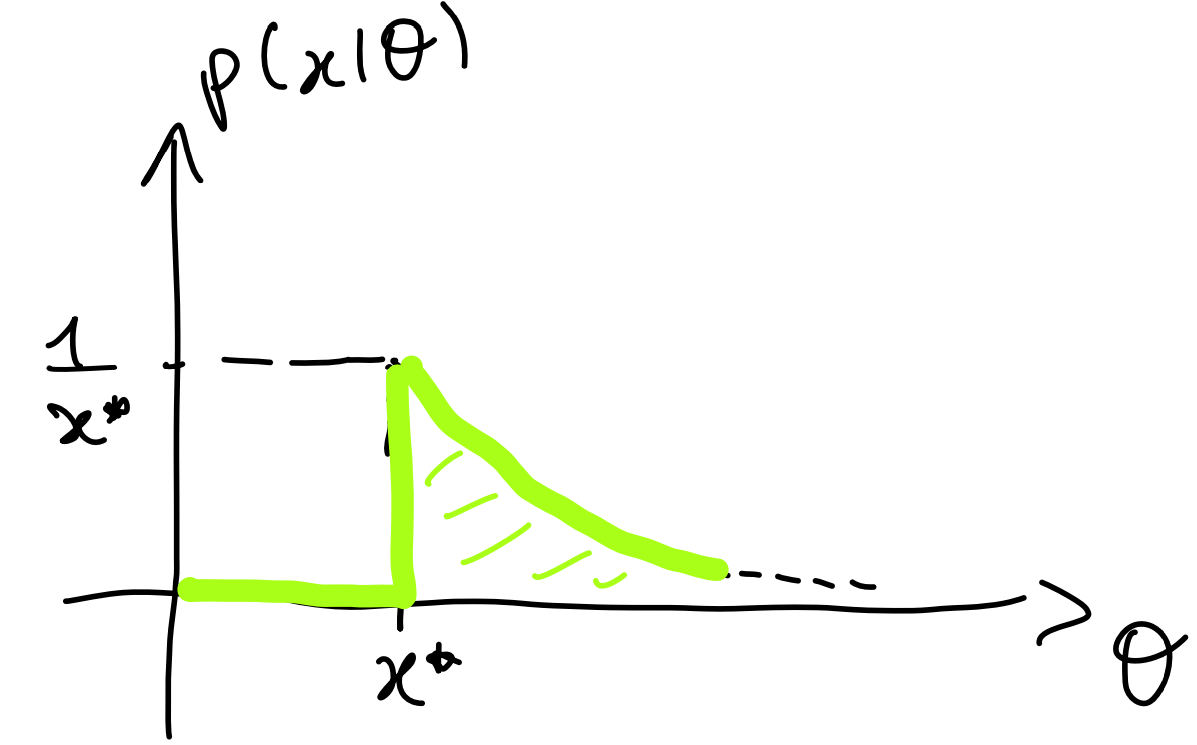
\includegraphics[scale=0.35]{B_7}
    \centering
\end{figure}
Being the dataset \(X=\{x_i|i=1,...,n\}\), the a-posteriori probability is:
\begin{align*}
    p(\theta|X)=\frac{p(X|\theta)p(\theta)}{p(X)}
    \propto
    p(X|\theta)=L(\theta|X)=\prod_{i=1}^{n}p(x_i|\theta)
\end{align*}
Thus, the likelihood is written as:
\begin{align*}
    L(\theta|X)=\prod_{i=1}^{n}\frac{1}{\theta}=\biggl(\frac{1}{\theta}\biggr)^{n}
\end{align*}
The likelihood is maximized when \(\theta\) is minimized, meaning that \(\theta\)
should be equal to \(x*\), which must be the largest of the \(x_i\) values,
otherwise at least one factor of the product is 0, leading to a null likelihood.
As a consequence, the maximum likelihood estimator \(\hat{\theta}\) can
only be \(\hat{\theta}=\max_{i}x_i\).